\documentclass{article}
\usepackage{graphicx}
\usepackage{float}

\title{CMSC6950 Project Report: Tidynamics}
\author{Karina Barcelos}
\date{Spring - June 2021}

\setlength{\oddsidemargin}{0.5cm}
\setlength{\textwidth}{15.5cm}
\setlength{\topmargin}{-1.5cm}
\setlength{\textheight}{22cm}

\begin{document}
\maketitle

\section{Introduction}

Tidynamics \cite{Buyl2018} calculates mean-square displacements (MSD) of a trajectory and correlation functions of input data using the Fast Correlation Algorithm. This package is beneficial for quantitatively evaluating dynamics of stochastic and molecular simulations from numerical trajectories, which depends only on Python and NumPy (utilizing arrays). 

The aim of this project was to implement two computational tasks of dynamical systems from a chosen open source package such as tidynamics\cite{Buyl2018}. For the first task, the autocorrelation funtion was computed for the bond length of C-H and C=O over 700 ns of a Molecular Dynamics (MD) simulation from a certain Tyrosine amino acid. For the second task,a random walk values and its mean-square displacement were generated. Several modules were utilized during the project, including, numpy, pandas, math, sys, and matplotlib. 

\section{Results}

Text

\subsection{Task 1}

Text 

\begin{figure}[H]
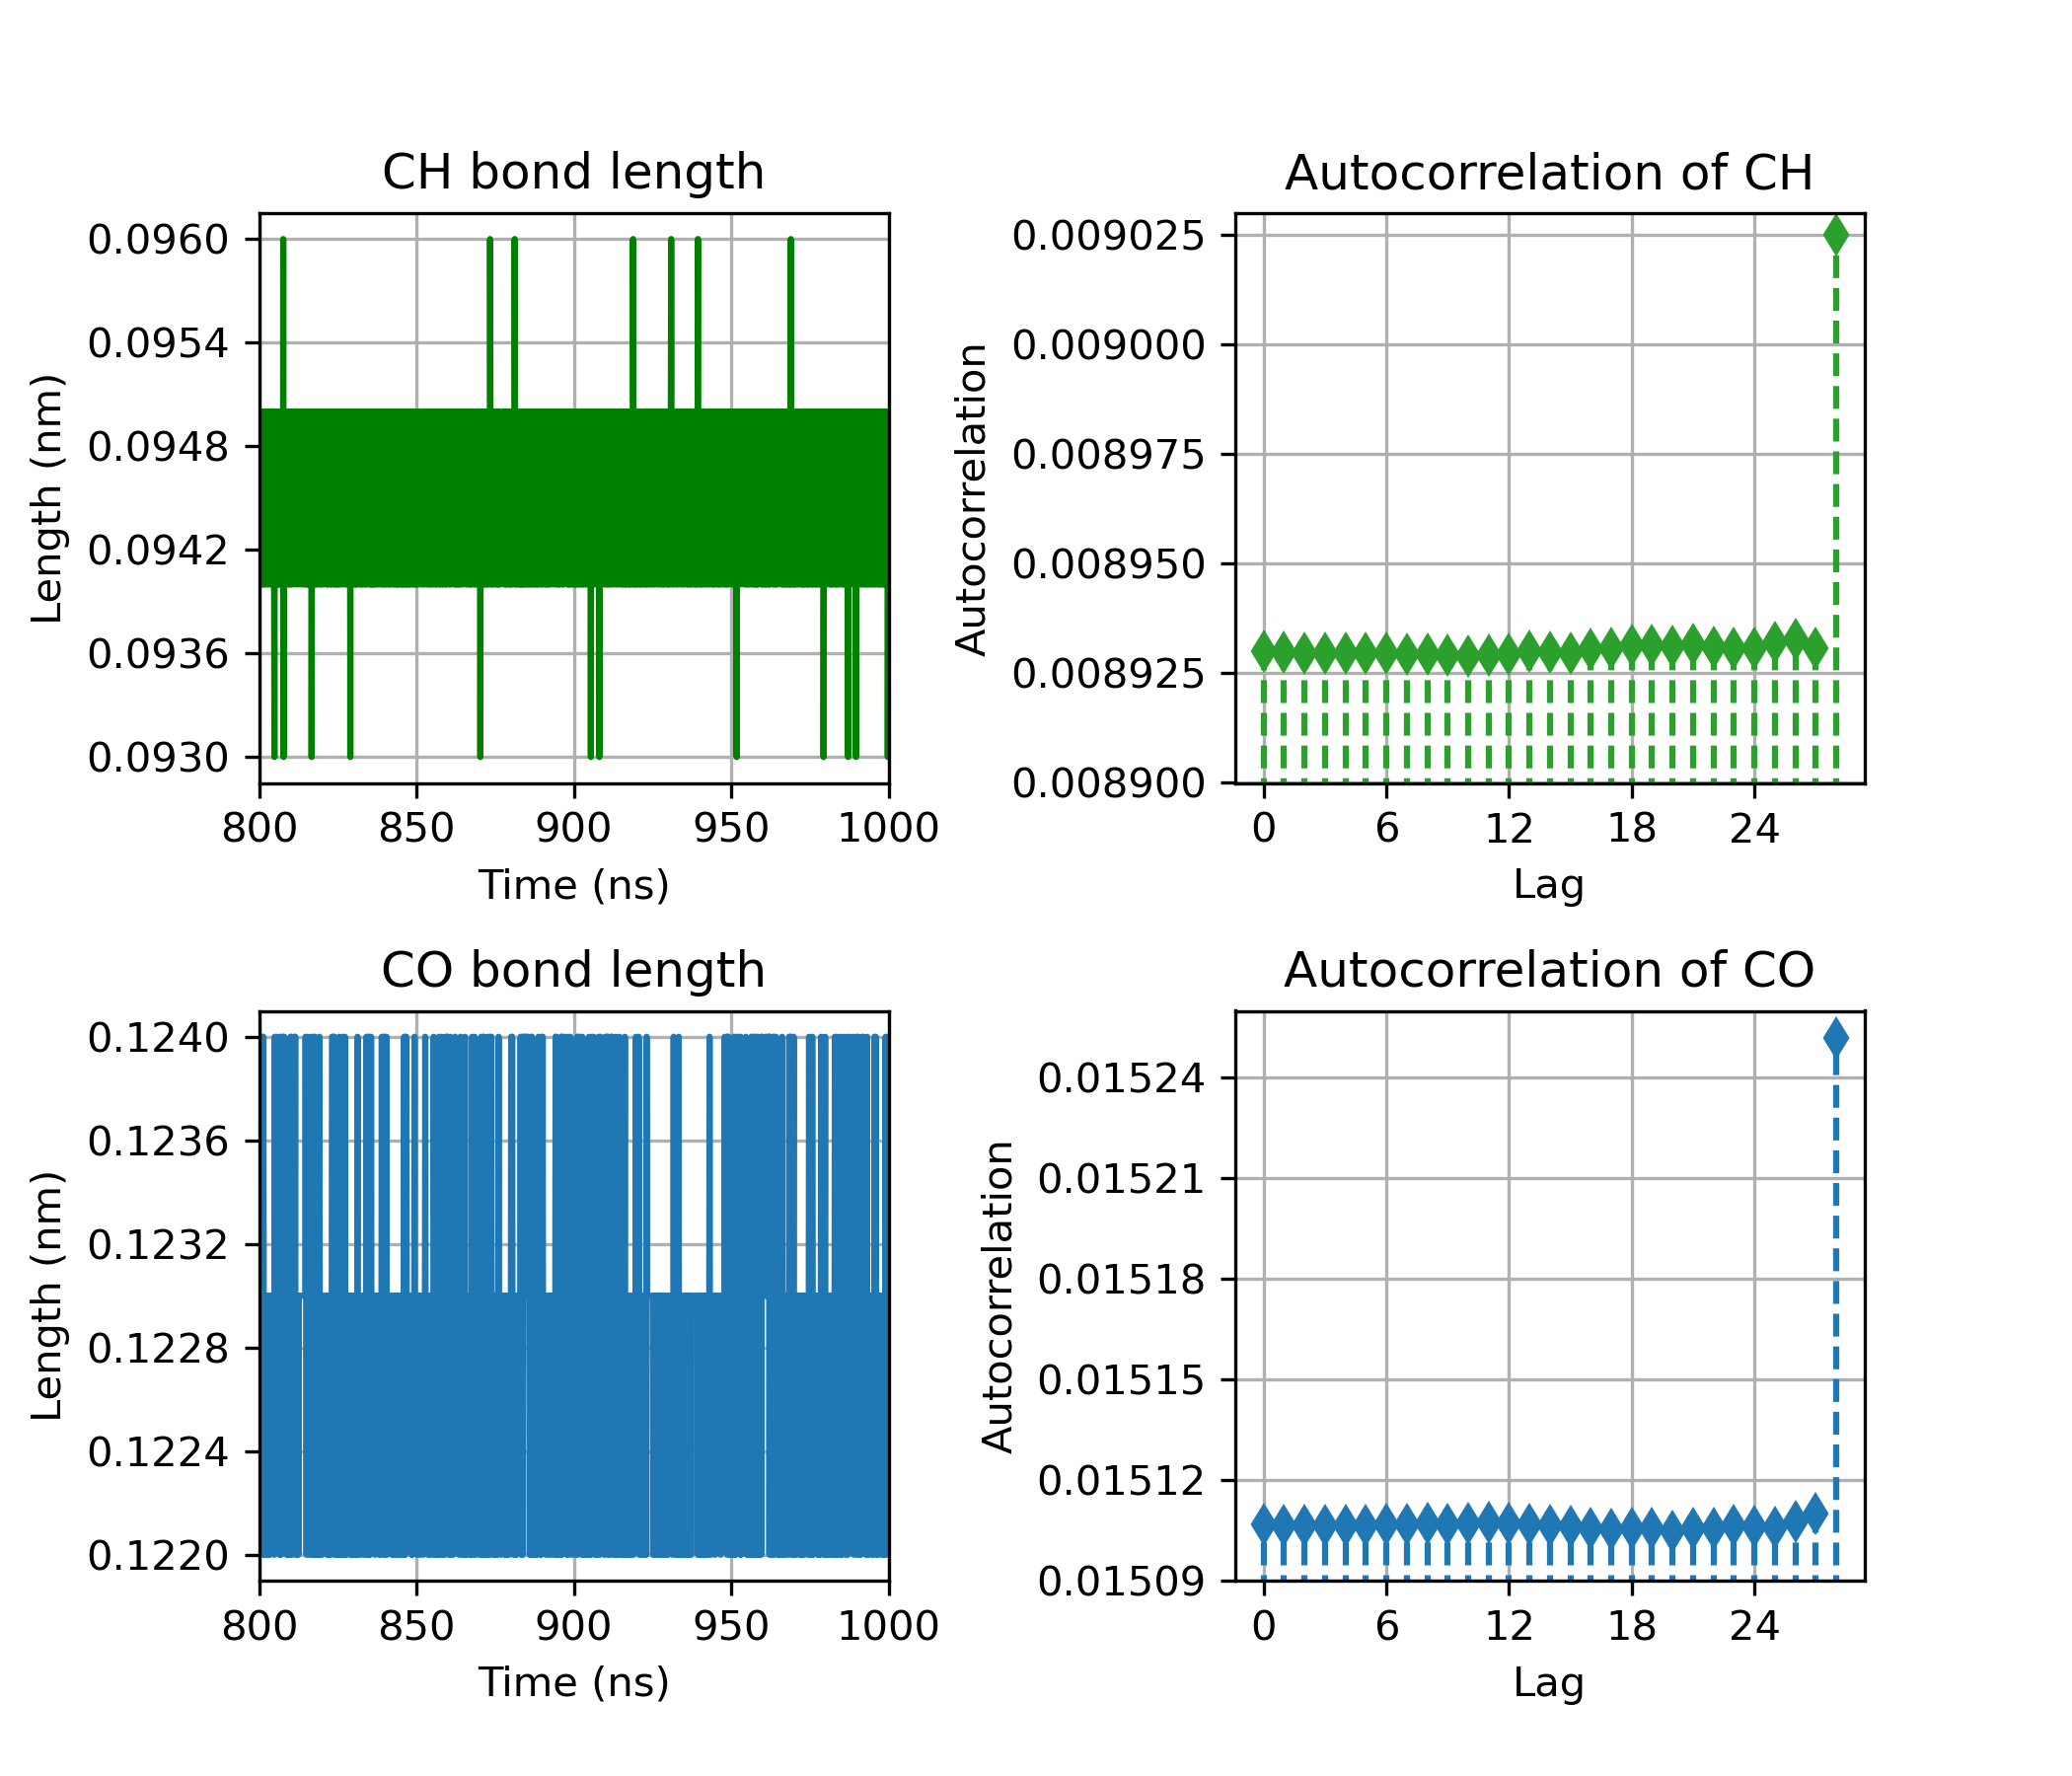
\includegraphics[width=\linewidth]{CO_CH_length_acf_plot.png}
\caption{XXC-H and C=O bond length over Molecular Dynamics time and their autocorrelation function.}
\label{acf_plot}
\end{figure}




\subsection{Task 2}


Text

\begin{figure}[H]
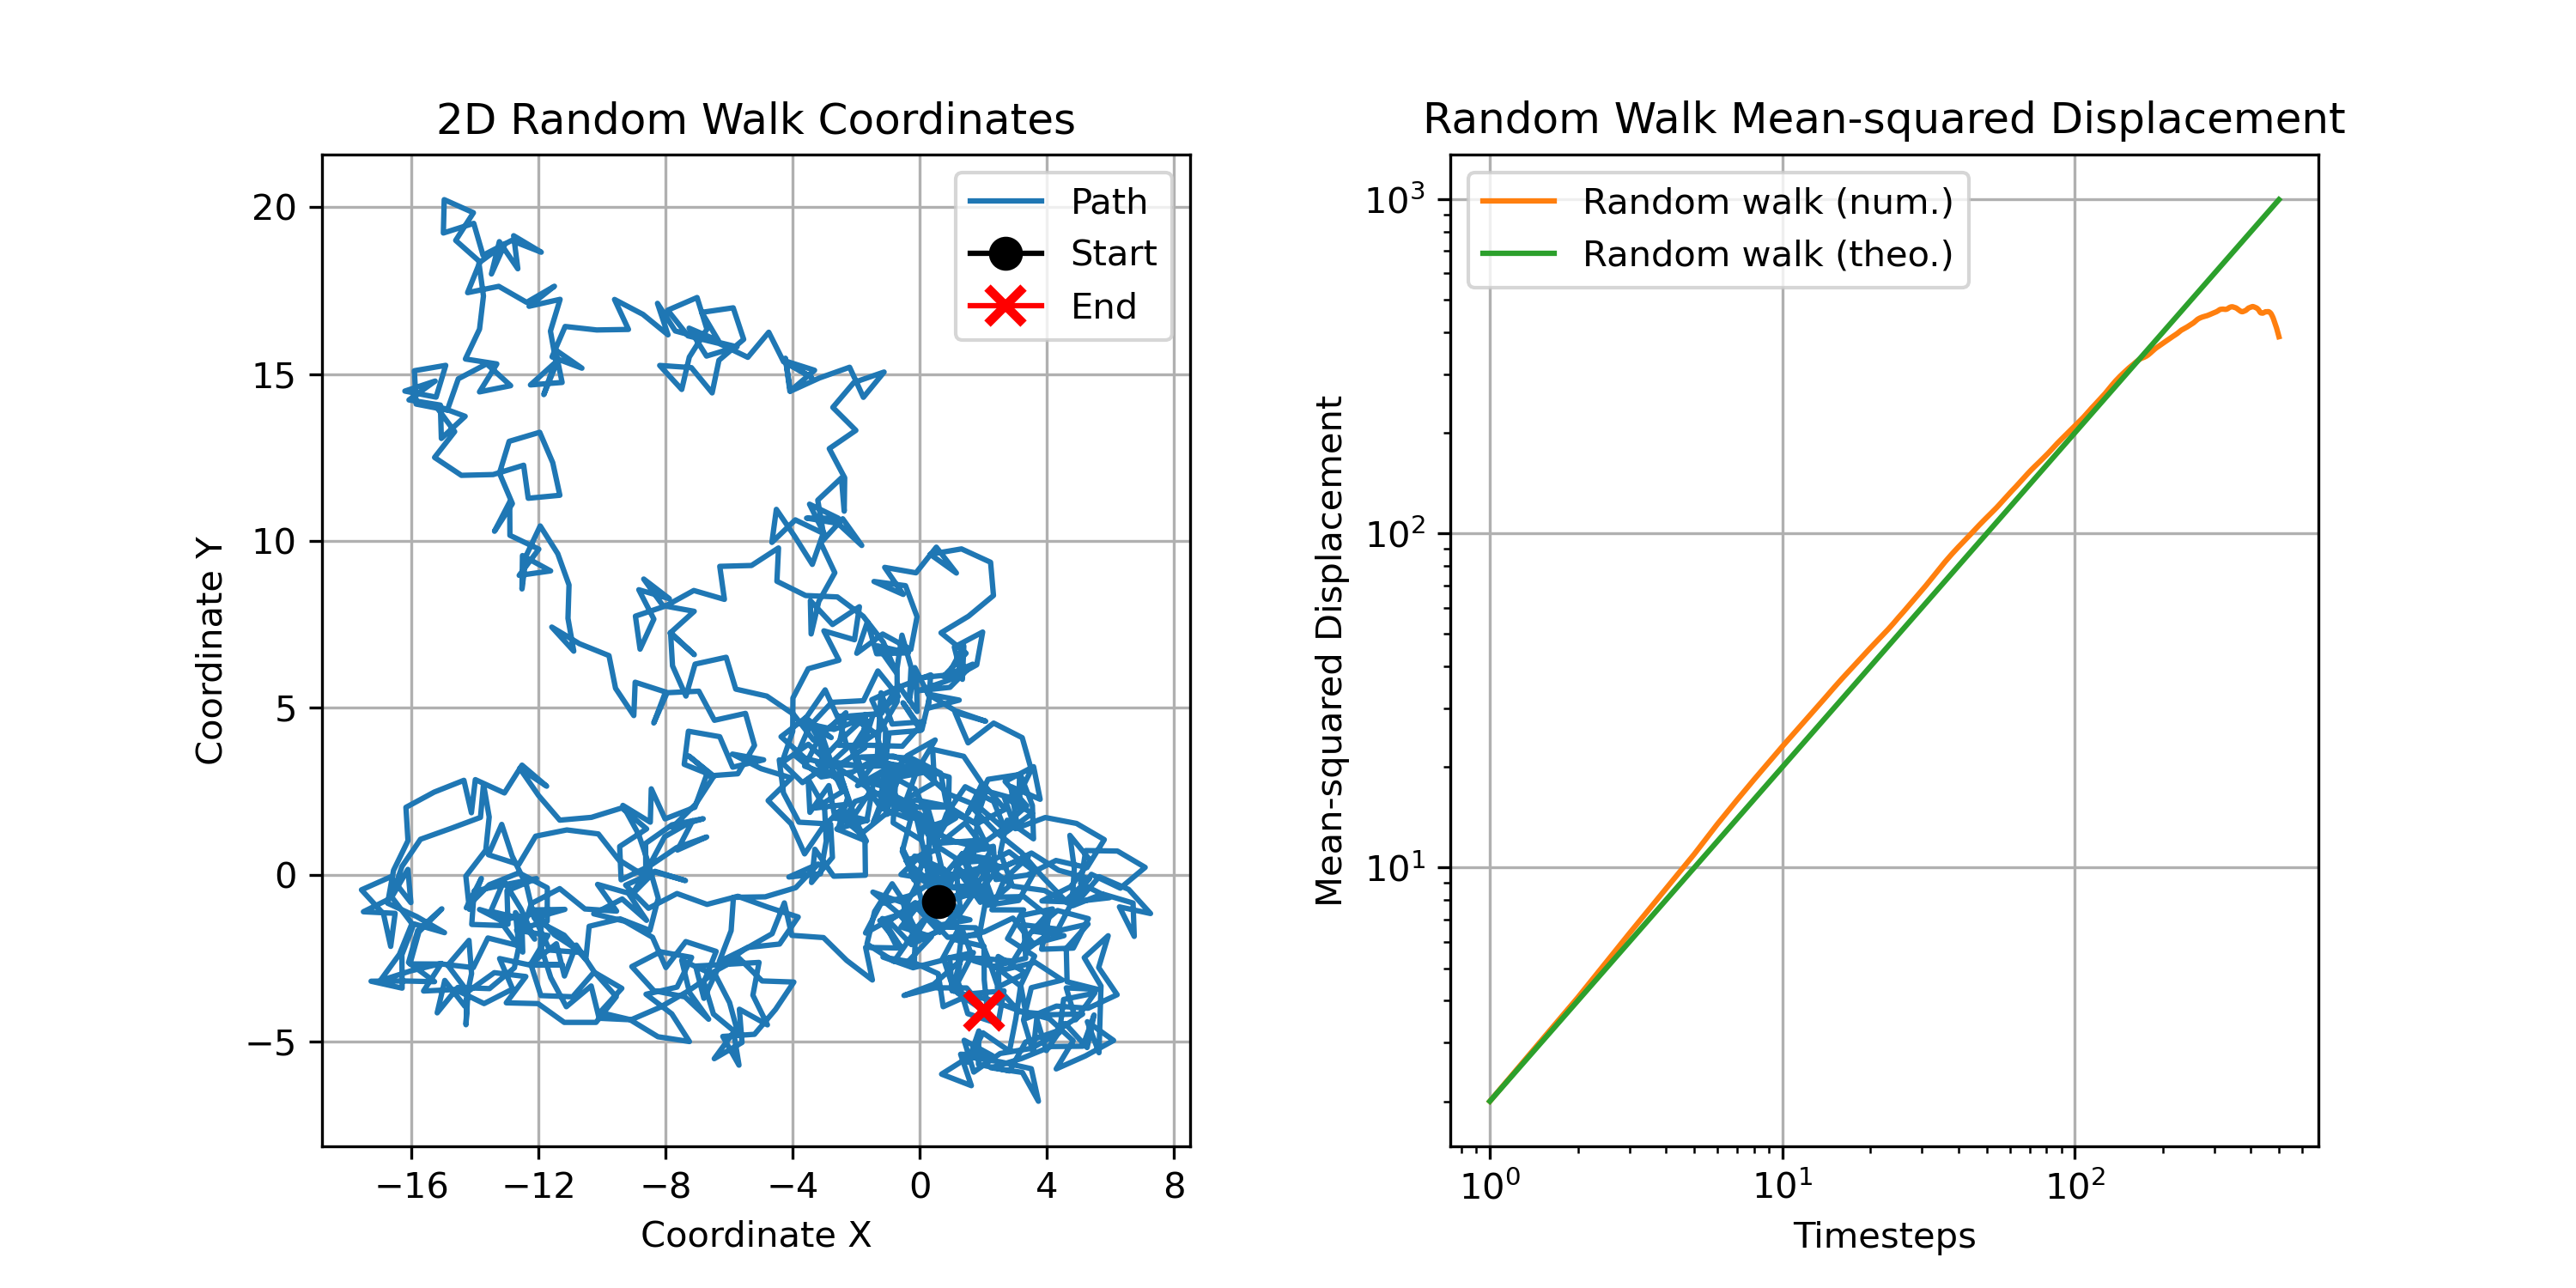
\includegraphics[width=\linewidth]{msd_plot.png}
\caption{2D random walk in a (x,y) coordinates and its mean-squared displacement.}
\label{msd_plot}
\end{figure}



\section{Conclusions}


\bibliography{refs}

\end{document}


\bibliographystyle{plain}
\bibliography{references}


\end{document}
